\documentclass[screen, aspectratio=43]{beamer}
\usepackage[T1]{fontenc}
\usepackage[utf8]{inputenc}

% Use the NTNU-temaet for beamer 
% \usetheme[style=ntnu|simple|vertical|horizontal, 
%     language=bm|nn|en, 
%     smalltitle, 
%     city=all|trondheim|alesund|gjovik]{ntnu2017}
\usetheme[style=ntnu,language=en]{ntnu2017}

\usepackage[english]{babel}
\usepackage[style=numeric,backend=biber,natbib=false,sorting=none]{biblatex}

\title[AP-intro]{MCT4048: Audio Programming}
\subtitle{The Extensions: Live Coding}
\author[A. Xamb{\'o}]{Anna Xamb{\'o}}
\institute[NTNU]{Department of Music, NTNU}
\date{13 February 2019}
%\date{} % To have an empty date

\addbibresource{../ap.bib} % Add bibliography database

% Set the reference style to numeric.
% See here: http://tex.stackexchange.com/questions/68080/beamer-bibliography-icon
\setbeamertemplate{bibliography item}[text] 

% Set bibliography fonts to a small size.
\renewcommand*{\bibfont}{\footnotesize}

\begin{document}

\begin{frame}
  \titlepage
\end{frame}

% Alternatively, special title page command to get a different background
% \ntnutitlepage
%
\begin{frame}
\frametitle{Start setting up...}
Download: \url{https://github.com/axambo/audio-programming-workshop/} 
\\
\vspace{10 mm}
Go to: \textrm{code/d6/00-setting-up/checklist.md}
\end{frame}
%
\begin{frame}
\frametitle{Reflecting on The Blogposts}
\end{frame}
%
\begin{frame}
\frametitle{This Week: The Extensions (40\% Group Work)}
\begin{itemize}
\item \textbf{Syllabus}: \url{https://uio.instructure.com/courses/17406}
\item \textbf{Assignment 4} (Total grade: 30\%): Presentation mini-project 2 (group) -- \textbf{\textcolor{olive}{days 6 (February 13, 2019) (10\%)}}, 7 (February 14, 2019) (10\%), 8 (February 15, 2019) (10\%)
\item \textbf{Assignment 5} (Total grade: 10\%):  Written blog post about the mini-project 2 (group) -- February 22, 2019
\end{itemize}
\end{frame}
%
\begin{frame}
\frametitle{Program: Day 6 -- 13 February, 2019}
\begin{itemize}
\item 9.15-10.00: Setting up computers with the tools for the tutorial
\item 10.00-12.30: Tutorial: Live coding
\item 12.30-13.00: Lunch break
\item 13:00-15:00: Mini-project 2 development (2/4)
\item 15.00-16.00: Speedy presentations mini-project 2 (1/3)
\end{itemize}
\end{frame}
%
\begin{frame}
\frametitle{Warm-up Activity: What Do We Know About Live Coding?}
\end{frame}
%
\begin{frame}
\frametitle{Mini-Presentation: Live Coding}
\begin{itemize}
\item Around SuperCollider and the Live Coding community.
\item Around collaborative music live coding.
\end{itemize}
\end{frame}
%
\begin{frame}
\frametitle{What is Gibber.cc}
\begin{itemize}
\item Gibber is a creative coding environment for audiovisual performance and composition. 
\item It contains features for audio synthesis and musical sequencing as well as drawing capabilities (2d and 3d).
\item To execute a line of code, place your cursor on it and hit Ctrl+Enter (line or block of code).
\end{itemize}
\end{frame}
%%
\begin{frame}
\frametitle{Live Coding with Gibber.cc}
\begin{itemize}
\item Exploration of Gibber.cc (individual): report to the group one discovery using Gibber.cc in the browser.
\item Exploration of Gibber.cc (small group): explore ways of collaborating using Gibber.cc in the browser.
\item Group improvisations using Gibber.cc in the browser.
\end{itemize}
\end{frame}
%
\begin{frame}
\frametitle{Learning Outcomes}
\begin{itemize}
\item Get a sense of live coding as a musical practice.
\item Get familiar with live coding in the browser focusing on collaborative live coding.
\item Be able to work in a group project relating audio programming concepts and building up from previous knowledge.
\item Be aware of best practices in web development in group projects.
\end{itemize}
\end{frame}
%
\begin{frame}
\frametitle{Organization of groups: Brainstorming}
   \begin{figure}
	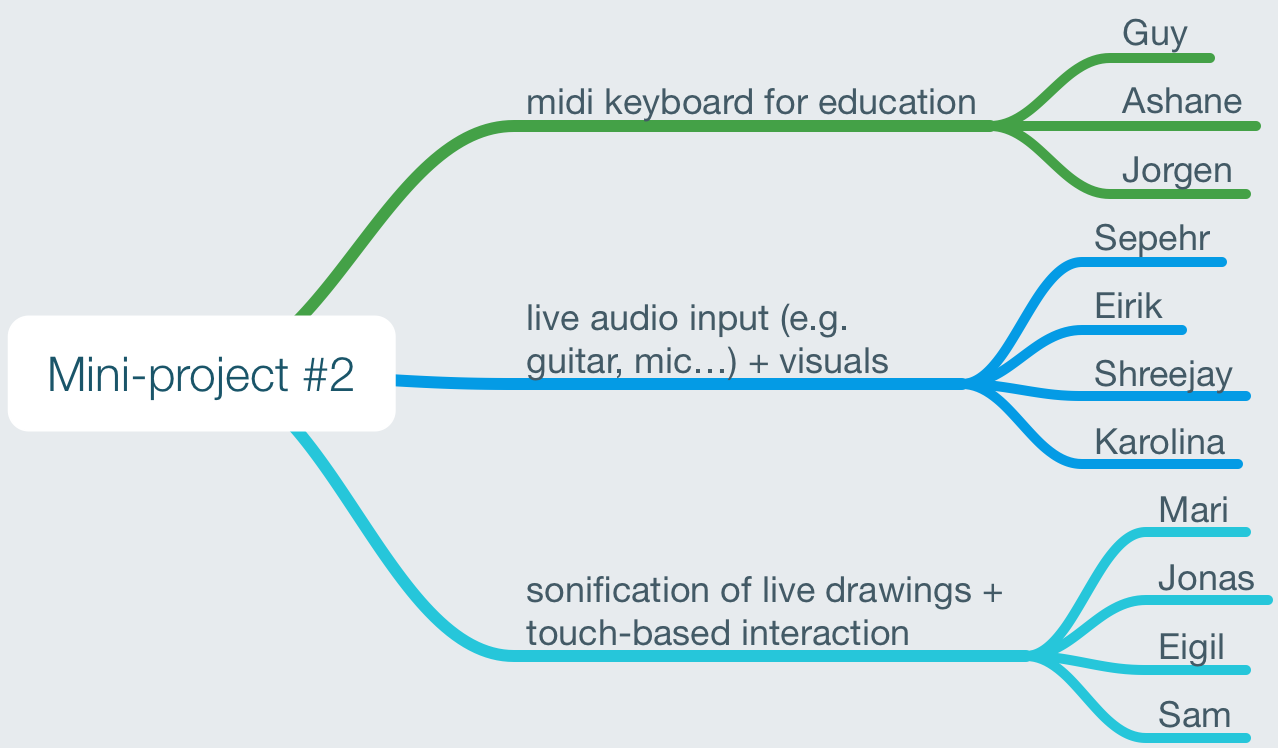
\includegraphics[scale=0.4]{img/groups-mini-project-2.png}
   \end{figure}
\end{frame}
%
\begin{frame}
\frametitle{Mini-project development (2/4)}
You are expected to create a mini-project in teams that should be doable within a week. The overall aim is to explore a little bit further Web Audio. Here are different approaches that you can take:
\begin{itemize}
\item Develop an idea based on what we are seeing in class. Feel free to build up everyday, or change if not convinced (from scratch approach).
\item Adapt an existing code to your needs and document what are the changes (remake approach).
\item Combine projects from last week (hybrid approach).
\item Other?
\end{itemize}
\end{frame}
%
\begin{frame}
\frametitle{Working style}
\begin{itemize}
\item Work with the same team throughout the week, ideally across campuses. 
\item Make sure to clarify who has developed what part of the code. For example, divide the work into functions and add the author name at the header of each function.
\item The instructors in both sites will keep an eye on the groups to catch up.
\item There will be 4 time slots during the week to work on the project. 
\item Keep a research journal.
\end{itemize}
\end{frame}
%
\begin{frame}
\frametitle{Relevant Links}
\begin{itemize}
\item Syllabus: \url{https://uio.instructure.com/courses/17406/pages/syllabus}
\end{itemize}
\end{frame}
%
%\begin{frame}
%  \frametitle{References}
%  \printbibliography
%\end{frame}
%
\end{document}
